\section{Application of Shielding Techniques in TEM Cells}\label{sec:shielding-sim}
\subsection{ASTM ES7-83 method}
\FloatBarrier

A model as described in \autoref{sec:astm} is used to determine the shielding effectiveness of nickel and zink according to the ASTM ES7-83 method discussed in \cref{sec:astm}. The TEM cell contains a shielding material sheet of thickness ranging from 1 to 40\,µm in the center of the TEM cell at $z=0$. A reference power $P_\mathrm{ref}=1\,\mathrm{W}$ is chosen, the load power $P_\mathrm{load}$ is numerically derived. Using \autoref{eqn:SE_power} yields the shielding effectiveness $SE_\mathrm{dB}$ of the material depending on thickness. The investigated frequency is 1\,GHz.

%\todo[inline]{Compare results with other papers}

\begin{figure}
	\centering
	\includegraphics[width=1\linewidth]{content/img/se}
	\caption{Shielding effectiveness of a sheet of zinc and nickel versus the material thickness determined with the ASTM ES7-83 Method.}
	\label{fig:se}
\end{figure}

%Metallic thin shields are normally removed from the computational domain and replaced by impedance network boundary conditions on the surfaces of the shielding material \cite{1430946}. Alternatively, the inside of the shielding material contains a fine mesh created with the adaptive meshing algorithm discussed in \cref{sec:simulations}, which is applied to these simulation models. 

\begin{table}[h]
	\centering

	{\renewcommand{\arraystretch}{1.2}
		\setlength{\tabcolsep}{12pt}
		\begin{tabular}{|l|c|c|c|}
			\hline
			Material & Rel. permittivity $\varepsilon_r$ & Rel. permeability $\mu_r$ & Conductivity $\sigma$ \\
			\hline\hline
			Zinc & $\approx 1$ & $\approx 1$ & $1.67 \cdot 10^7$\,S/m\\
			\hline
			Nickel & $\approx 1$ & $600$ & $1.45 \cdot 10^7$\,S/m \\
			\hline
			Permalloy 45 & $\approx 1$ & $\approx 90,000$ & $2.00 \cdot 10^6$\,S/m\\
			\hline
			Barium titanate & $\approx 2,000$ & $\approx 1$ & $3.64\cdot 10^{-11}$\,S/m \\
			\hline
	\end{tabular}}
	\caption{Electromagnetic Properties of Zinc and Nickel}
	\label{tab:materials}
\end{table}

\subsection{Dual TEM cell}

A simulation model of two TEM cells as shown in \autoref{fig:dual_tem_cell}, consisting of the models demonstrated in \cref{sec:tem_cell_model}, without the tapered sections, is created. An empty square aperture with a side length of $d=10\,\mathrm{mm}$ is used, which makes it electrically small up to a frequency of approximately $3\,\mathrm{GHz}$. The largest numerical error stems from insufficient mesh size in the aperture region, hence 10 to 15 mesh elements across the aperture are aimed for. The procedure described in \cref{sec:dual_tem_cell} is applied to derive the electric and magnetic shielding effectiveness of permalloy 45 and barium titanate.

Port 1 excites the waveguides with a power of $1\,\mathrm{W}$. The sum  $P_\mathrm{ref,sum}$ and difference $P_\mathrm{ref,diff}$ of the powers arriving at port 3 and 4 is demonstrated in \autoref{fig:emptypowersumdiff}. 

%Simulation model leans on measurement setup in \cite{4091811}.

%\begin{figure}[htbp]
%	\centering
%	\includegraphics[width=1\linewidth]{content/img/empty-aperture-coupling}
%	\caption{Coupling of port 1 to ports 3 and 4 with empty square aperture}
%	\label{fig:empty-aperture-coupling}
%\end{figure}

\begin{figure}[htbp]
	\centering
	\includegraphics[width=1\linewidth]{content/img/empty_power_sum_diff}
	\caption{The sum $P_\mathrm{ref,sum}$ and difference $P_\mathrm{ref,diff}$ of the reference power, measured with empty aperture and calculated with the phase information considered.}
	\label{fig:emptypowersumdiff}
\end{figure}

Materials filling the aperture have a thickness of $t=10,\upmu\mathrm{m}$. For highly conductive materials, applying skin-depth based meshing within the material enhances accuracy while reducing computational effort. This approach refines the mesh especially near the material’s surface, where rapid field variations occur. The skin depth is calculated as shown in \autoref{eqn:skin_depth} and further discussed in \cref{sec:skin_effect}. Again, the sum $P_\mathrm{ref,sum}$ and difference $P_\mathrm{ref,diff}$ of the powers at port 3 and 4 are derived and shown in \cref{fig:bariumpowersumdiff,fig:permalloypowersumdiff}, once for the aperture filled with barium titanate, and once with permalloy 45.

\begin{figure}[htbp]
	\centering
	\begin{subfigure}[b]{0.48\textwidth}
		\centering
		\includegraphics[width=1\linewidth]{content/img/barium_power_sum_diff}
		\caption{Barium titanate}
		\label{fig:bariumpowersumdiff}
	\end{subfigure}
	\hfill
	\begin{subfigure}[b]{0.48\textwidth}
		\centering
		\includegraphics[width=1\linewidth]{content/img/permalloy_power_sum_diff}
		\caption{Permalloy 45}
		\label{fig:permalloypowersumdiff}
	\end{subfigure}
	\caption{The sum $P_\mathrm{load,sum}$ and difference in output power $P_\mathrm{load,diff}$ measured at port 3 and 4 with the phase information considered.}
	\label{fig:example}
\end{figure}

Permalloy 45 exhibits lower power transfer, indicating stronger shielding effectiveness compared to barium titanate. Additionally, $P_\mathrm{load,sum}$ is low for both materials, suggesting high electric shielding effectiveness, as indicated by \cref{eqn:se_dual_cell_e}. When the aperture is filled with barium titanate, power transfer increases with frequency, which can be attributed to the material’s low bulk conductivity and slightly decreasing permittivity at higher frequencies. In contrast, the transferred power through the permalloy 45 sheet decreases with frequency, reflecting increased absorption due to the material’s high bulk conductivity. The electric and magnetic shielding effectiveness for both materials are illustrated in \cref{fig:sebarium,fig:sepermalloy}.

\begin{figure}[htbp]
	\centering
	\begin{subfigure}[b]{0.48\textwidth}
		\centering
		\includegraphics[width=1\linewidth]{content/img/se_barium}
		\caption{Barium titanate}
		\label{fig:sebarium}
	\end{subfigure}
	\hfill
	\begin{subfigure}[b]{0.48\textwidth}
		\centering
		\includegraphics[width=1\linewidth]{content/img/se_permalloy}
		\caption{Permalloy}
		\label{fig:sepermalloy}
	\end{subfigure}

	\caption{The electric $SE_\mathrm{dB}^\mathrm{e}$ and magnetic $SE_\mathrm{dB}^\mathrm{m}$ shielding effectiveness derived with \cref{eqn:se_dual_cell_e,eqn:se_dual_cell_m}.}
	\label{fig:se_e_m}
\end{figure}

\todo[inline]{TODO: Permalloy 45 simulationergebnis ist unpräzise im niedrigen Frequenzbereich, ich werde das ausbessern.}

Barium titanate exhibits good electric shielding characteristics, but demonstrates a negative $SE_\mathrm{dB}^\mathrm{m}$ value, indicating poor magnetic shielding. This effect occurs due to interference patterns at the filled aperture, which cause port 3 to receive more power, than in the case of an empty aperture \cite{4091811}.

Barium titanate has a high permittivity, which is related to high electric shielding, but low bulk conductivity and permeability, as shown in \autoref{tab:materials}. Consequently, magnetic shielding is low. 

\subsection{Antennas in shielding enclosures}

The loop and monopole antennas investigated in \cref{sec:monopole,sec:loop_sim} are shielded in a covered enclosure, as shown in \cref{fig:loopantennaenclosure,fig:monopoleantennaenclosure}. The enclosure has a thickness of $10\,$µm, and all sides have a length of 6\,mm. The near-field region of the monopole antenna is predominantly electric (\autoref{eqn:compl_power_inf_elec_dipole}), while that of the loop antenna is magnetic (\autoref{eqn:pr_loop}).

\begin{figure}[htbp]
	\centering
	\begin{subfigure}[t]{0.48\textwidth}
		\centering
		\includegraphics[width=1\linewidth]{content/img/loop_antenna_enclosure}
		\caption{Loop antenna}
		\label{fig:loopantennaenclosure}
	\end{subfigure}
	\hfill
	\begin{subfigure}[t]{0.5\textwidth}
		\centering
		\raisebox{1.5mm}{\includegraphics[width=1\linewidth]{content/img/monopole_antenna_enclosure}}
		\caption{Monopole antenna}
		\label{fig:monopoleantennaenclosure}
	\end{subfigure}
	
	\caption{Investigated antennas placed in the TEM cell covered in a cubic enclosure.}
	\label{fig:example}
\end{figure}

\autoref{fig:bariumenclosurepower} shows the radiated power by the antennas with and without barium titanate enclosure. The output power increases due to the barium titanate enclosure capacitively loading the antenna. This leads to an decrease in resonance frequency, making it a more efficient radiator at the investigated frequency range, as discussed in \autoref{sec:loop_sim}. 

\begin{figure}
	\centering
	\includegraphics[width=1\linewidth]{content/img/barium_enclosure_power}
	\caption{Barium titanate}
	\label{fig:bariumenclosurepower}
\end{figure}



\FloatBarrier
%\subsection{Shielding Antennas}
%
%\todo[inline]{shielding antennas and investigating field distribution will be done here. Some tilt in shielding material would be interesting to investigate}
%
%\subsection{Shielding Equivalent Dipole Moments}
%
%\todo[inline]{Check latex comments, which contain some good ideas. TODO Rest of section}

%\todo[inline]{Rest of shielding material section still TODO}
%\subsection{Shielding effectiveness of graphite}
%
%The reference power $P_\mathrm{ref}$ has been set to 1\,W. Using \autoref{eqn:load_power} and the S-parameters from the simulation results, $P_\mathrm{load}$ may be determined. \autoref{fig:se_graphite} demonstrates the shielding effectiveness of graphite in dB $SE_\mathrm{dB}$ over the shielding material thickness. The solution frequency is 500\,MHz. A frequency sweep shows that the reflection coefficient $S_{11}$ does not depend much on the frequency. 
%
%\begin{figure}[h]
%	\centering
%	\includegraphics[width=1\linewidth]{content/img/se_graphite.png}
%	\caption{Shielding effectiveness of graphite}
%	\label{fig:se_graphite}
%\end{figure}
%
%The components of $SE_\mathrm{dB}$ are determined according to \autoref{eqn:se_rereflections}. 
%
%\subsection{Shield effectiveness of FR4}
%
%The FR4 has a relative permittivity of $\epsilon_r=4.4$. According to \autoref{eqn:rel_wave_imp}, the relative wave impedance is $Z=0.476$. This leads to a reflection coefficient of $R=-0.355$ by \autoref{eqn:reflection_coefficient_plane_dielectric}.
%
%
%The reflection coefficient $|S_{11}|=0.045$.
%
%\subsection{Dual TEM Cell}
%
%A simulation setup of a dual TEM cell is created. A rectangular aperture with a side length of $l=5\,\mathrm{cm}$, inspired by \cite{Wilson_1981}, connects both TEM cells. One waveport 1, as in \autoref{fig:dual_tem_cell}, is excited with a power of $P=1\,\mathrm{W}$. The simulation is conducted, leaving the aperture open. A second one determines the coupling of the waveports, when the aperture is filled with a graphite sheet with a thickeness of $t=50$\,µm.
%
%At a frequency of $f=500\,\mathrm{MHz}$, the coupling between waveport 1 to the waveports 3 and 4 of the receiving TEM cell is shown in \autoref{tab:dual_tem_fwd_trans}. Only one frequency point is investigated, as the results stay roughly constant over the inspected frequency range from 100\,MHz to 1\,GHz. 
%
%
%\begin{table}
%	\centering
%	\begin{tabular}{|c|c|c|}
%		\hline
%		Forward transmission coefficient & Empty aperture & aperture filled with FR408\\\hline\hline
%		Waveport 1 to 3 $S_{13}$ & -83.80\,dB, -144.96° & -85.27\,dB, -155.79°\\\hline
%		Waveport 1 to 4 $S_{14}$ & -90.31\,dB, -144.96° & -87.14\,dB, 25.00°\\\hline
%	\end{tabular}
%	\caption{Forward transmission coefficients}
%	\label{tab:dual_tem_fwd_trans}
%\end{table}
%\todo{Why -8dB difference in empty aperture? Explained in \cite{Wilson_1981}}
%
%Using \autoref{eqn:se_dual_cell_e} and \autoref{eqn:se_dual_cell_m} leads to the shielding effectiveness for electric coupling $SE_\mathrm{dB}^\mathrm{e}=19.07\,\mathrm{dB}$ and magnetic coupling $SE_\mathrm{dB}^\mathrm{m}=-9.22\,\mathrm{dB}$. \todo{negative SE possible? Redo Simulations with finer Mesh around aperture} To get the sum $P_\mathrm{sum}$ and difference $P_\mathrm{diff}$ of powers, the phase of the signals have to be considered. With unit input power at the transmitting TEM cell, \autoref{eqn:s_param_to_power_sum} and \autoref{eqn:s_param_to_power_diff} are used for this purpose \cite{Sreenivasiah_Chang_Ma_1981}. 
%
%\begin{subequations}
%	\begin{equation}
%		P_\mathrm{sum} = (S_{13} + S_{14})(S_{13} + S_{14})^*
%		\label{eqn:s_param_to_power_sum}
%	\end{equation}
%	\begin{equation}
%		P_\mathrm{diff}= (S_{13} - S_{14})(S_{13} - S_{14})^*
%		\label{eqn:s_param_to_power_diff}
%	\end{equation}
%\end{subequations}
%
%Indicated by the phase shift of roughly 180°, the coupling between the TEM cells occur mainly due to magnetic dipoles. Due to the relative permittivity of $\epsilon _\mathrm{r}=3.66$ and the relative permeability of $\mu_r\approx 1$ of the shielding material, the magnetic fields dominate. This leads to a energy transfer mainly due to magnetic dipole moments\todo{One port receives overall more power due to the material. Is it because of the magnetic/electric dipoles in it? Check mesh around the small aperture.} The overall shielding effectiveness $SE_\mathrm{dB}=$ \autoref{eqn:dual_tem_cell_tot_power}.
%
%\begin{equation}
%	P_\mathrm{total}=|S_{13}|^2+|S_{14}|^2
%	\label{eqn:dual_tem_cell_tot_power}
%\end{equation}

% Show which dipole moments are affected by an offset in z-direction, and which ones are not.
